\section{Background}%1.5 pages  0.5pages/point
\label{sec:background}

\subsection{Sparsity in Transformer Models} 
\label{sec:transformer_sparsity}

\subsubsection{Transformer Structure} Transformer is a widely recognized DL structure, where each encoder or decoder contains multiple multi-head attention (MHA) layers~\cite{vaswani2017A}. The key operation of the MHA layer is scaled dot product attention (SDPA), which calculates the dot product of $Q$ and $K$, scales the result, optionally applies a mask at this stage, then applies the \texttt{Softmax} function to obtain the probabilities ($P$) and finally calculates the dot product of $P$ and $V$. Beyond MHA, Transformer includes downstream components: \texttt{Add} retains non-linear transformation information, \texttt{Norm} mitigates internal covariate shift via mean/variance normalization, and the \texttt{Feed Forward} layer comprises chained general matrix multiply (GEMM) operations with activations like \texttt{GELU} or \texttt{ReLU}. These components enable Transformer to handle complex cross-domain tasks while introducing operator characteristics that facilitate fusion-based optimizations.


%\vspace{-5pt}
\begin{figure}[htpb]
  \centering
  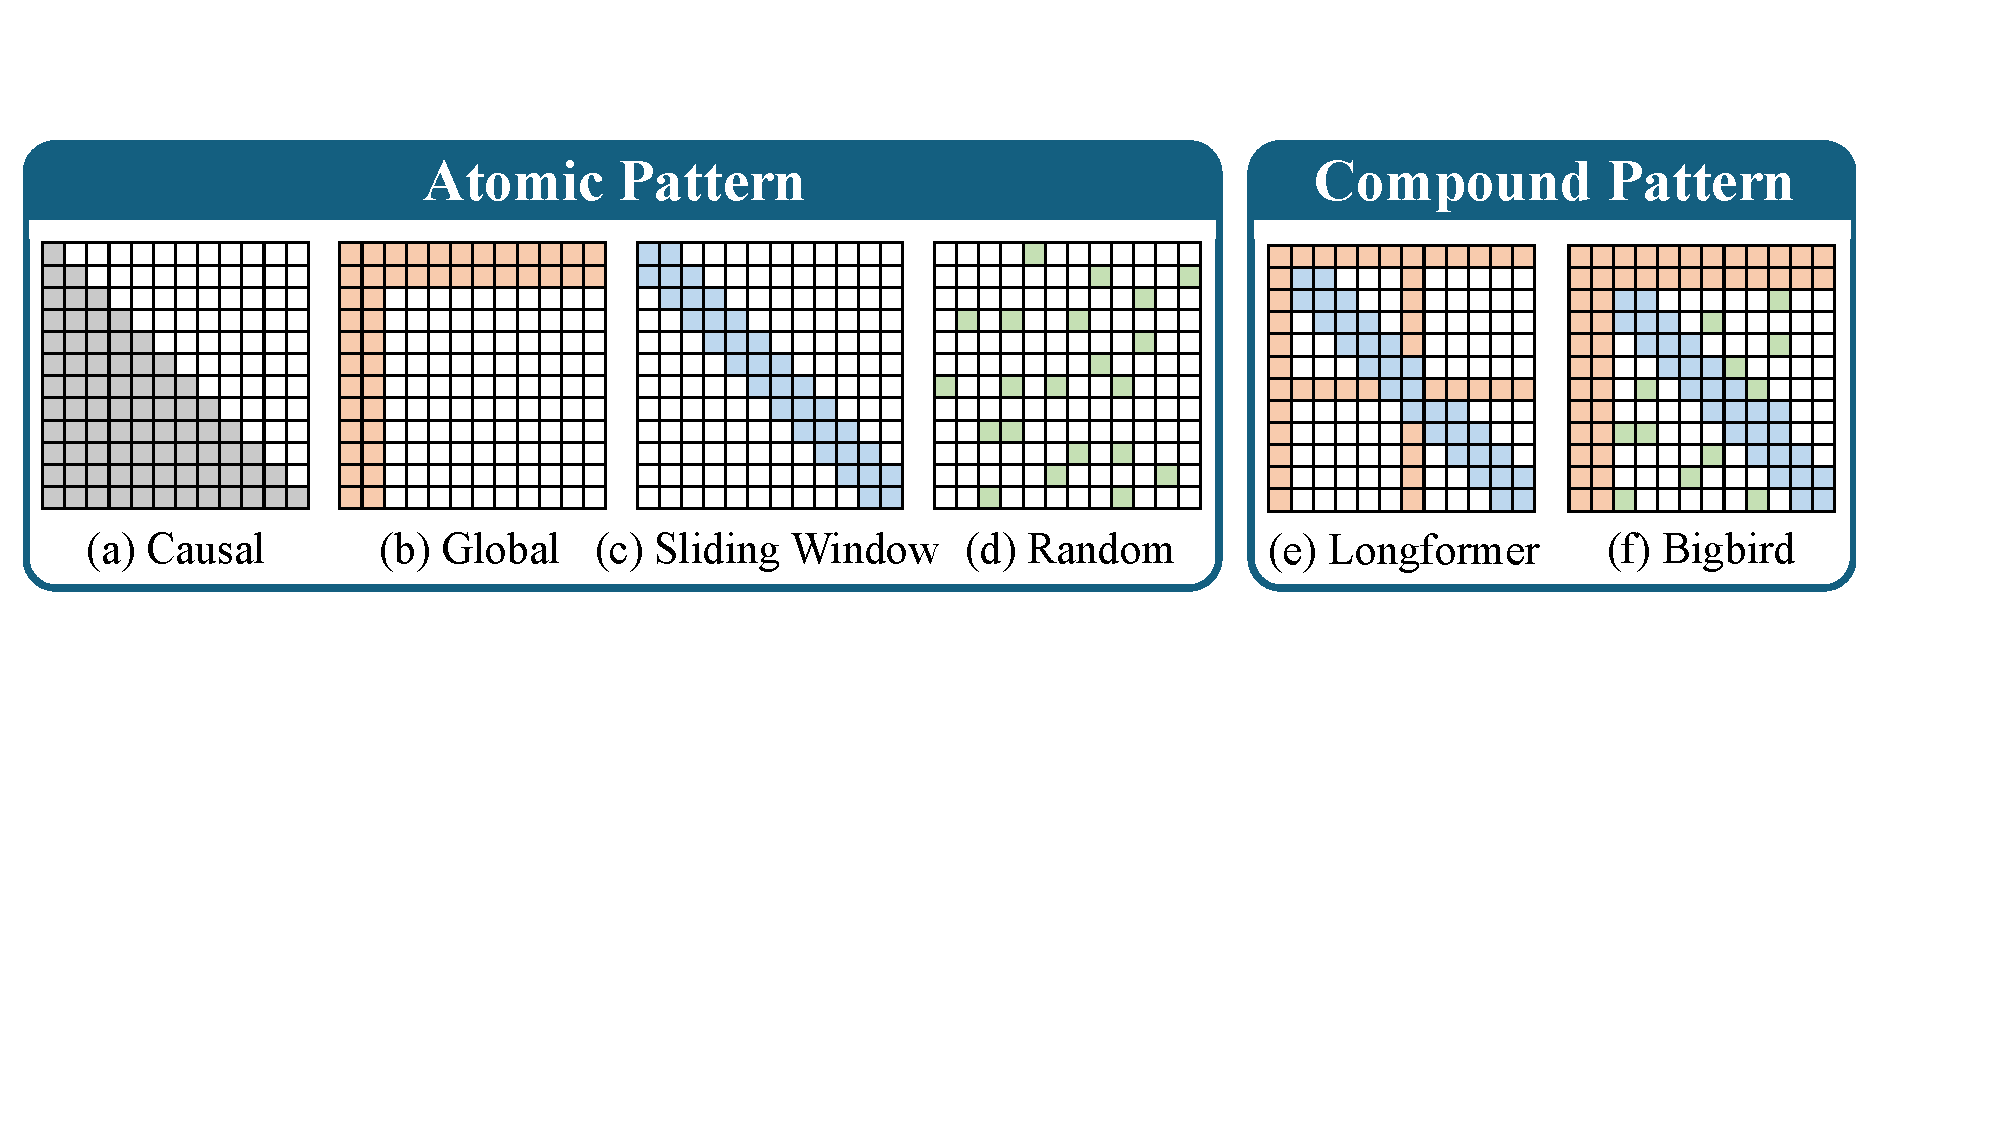
\includegraphics[width=\linewidth]{figures/2-bg-A-mask.pdf}
  %\vspace{-20pt}
  \caption{Atomic and compound sparse attention patterns.}
  \label{fig:bg-mask}
\end{figure}
%\vspace{-5pt}

\subsubsection{Sparse Attention Patterns}

Atomic sparse attention patterns are the building blocks of current popular sparse attention modules~\cite{adnan2024keyformer, liu2023deja, lin2022survey, roy2021efficient, beltagy2020longformer, zaheer2020big, child2019generating}. Figure~\ref{fig:bg-mask} (a)-(d) depict four most common atomic sparse attention patterns. The details are as follows.

\begin{itemize}
  \item \textit{Causal Attention.} To maintain temporal order, the query can access only preceding information, restricting connections to earlier nodes (the colored triangular).
    
  \item \textit{Global Attention.} Certain ``global'' nodes serve as central hubs, which receive information from others (the colored rows) and send it back (the colored columns).

  % DWH 预计去掉这一组 实验部分也换成 Causal 部分的
  % \item \textit{Dilated Attention.} Certain elements are skipped at a fixed stride to only process information of elements that have a periodic distribution (the colored hole-punched bands).
  
  \item \textit{Sliding Window Attention.} Considering the concept of locality, the query only focuses on the neighboring nodes within a defined window size, with its mask matrix presenting a banded pattern (the colored bands).
  
  \item \textit{Random Attention.} The query block is randomly associated with the preceding and following information. By adjusting the filling rate, it has the possibility to discover accidental correlations (the colored blocks).
\end{itemize}



% DWH: 我们的方式可以是一个 pass 的“形式”
% 自动与手动的根本区别在于能不能自动的发现 Attention 结构然后进行替换
% 虽然我们是手写的 CUDA kernel 
\subsection{Fused Kernel for MHA Structure}
\label{sec:kfam}


Numerous works~\cite{dong2024flex, wang2024flashmask,wang2024raptor,zhai2023bytetransformer,dao2022flashattention,wang2022lightseq2, fang2021turbotransformers,zheng2023chimera,zhang2024mcfuser,xFormers2022,nvidia22faster} have explored fusing MHA on GPU. Figure~\ref{fig:bg-fusion} shows a typical workflow of MHA fusion. The DL framework firstly parses the computational graph and captures the MHA sub-graph composed of coarse-grained native operators. Then, MHA fusion can be achieved manually or automatically. However, if the fusion of MHA with a certain mask layer is not supported, the sub-graph will be split into fine-grained meta operators to discover small-scale fusion opportunities.

% 2025.11.18 增加 SPLAT 后已重新刷新引用; 
%\vspace{-5pt}
\begin{figure}[htpb]
  \centering
  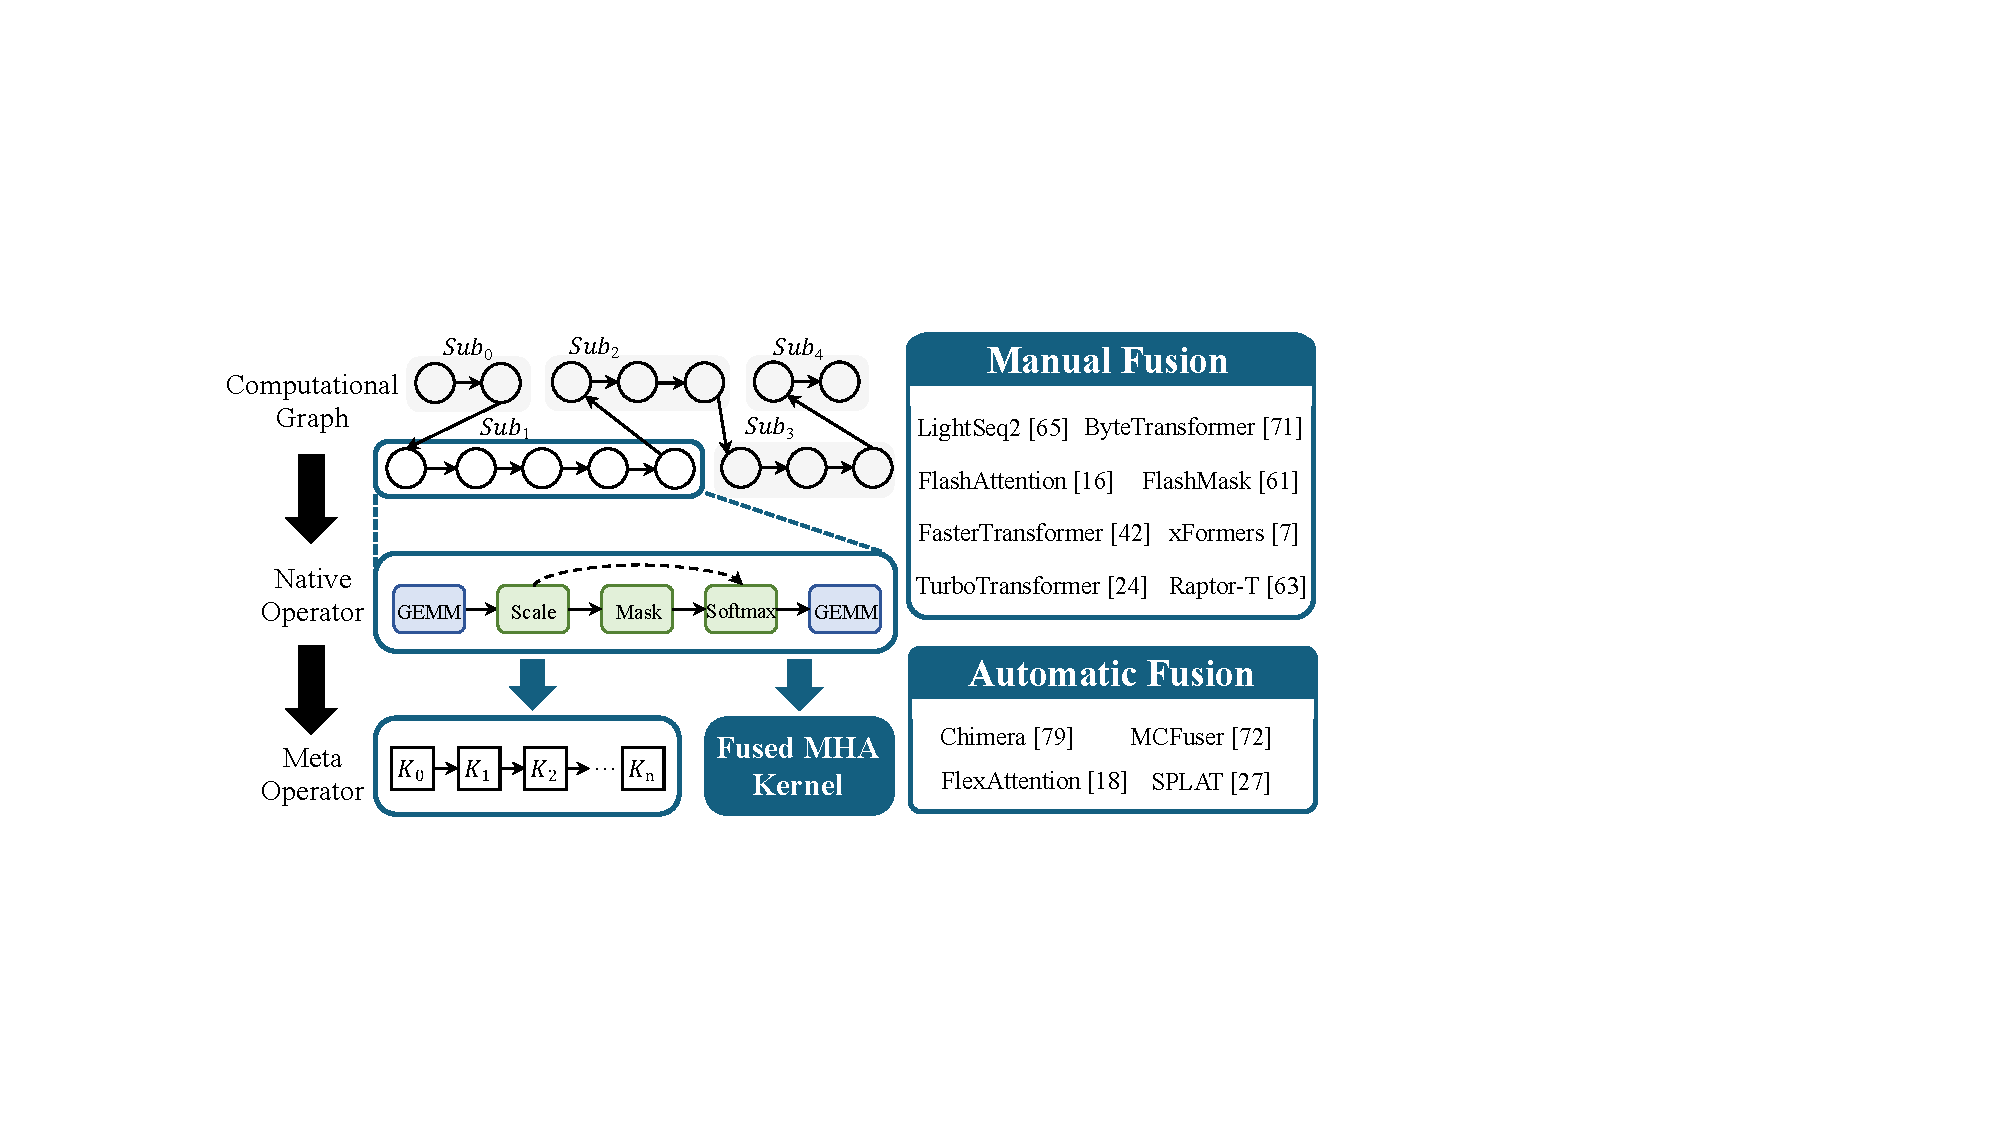
\includegraphics[width=\linewidth]{figures/2-bg-B-fusion.pdf}
  %\vspace{-5pt}
  \caption{Kernel fusion for MHA computation.}
  \label{fig:bg-fusion}
\end{figure}

Early works focus on the manual fusion of dense attention without the mask layer. %TurboTransformer~\cite{fang2021turbotransformers} processes element-wise operations in embarrassingly parallel. 
ByteTransformer~\cite{zhai2023bytetransformer} adopts hand-written kernels: short sequences store the intermediate matrix entirely in shared memory (SMEM) and registers; longer sequences employ grouped GEMM to ease resource constraint. The customized kernels limit ByteTransformer to a maximum sequence length of 1,024. FlashAttention (FA) series\footnote{FA3~\cite{shah2024flashattention3} is only for GPUs with Hopper architecture and later.} becomes the most typical open source implementation.
FA~\cite{dao2022flashattention} partitions the input into blocks and passes the blocks to SMEM multiple times, gradually performing \texttt{Softmax} reduction. FA2~\cite{dao2023flashattention2} further partitions the work between warps within one block of attention computation to reduce the read and write of SMEM. However, FA only supports common masking patterns such as causal and sliding window. FlashMask~\cite{wang2024flashmask} extends FA with column-wise representation to exploit attention sparsity for skipped computations, integrated into PaddlePaddle~\cite{ma2019paddlepaddle} but unable to represent discrete distributions such as random attention.


For automatic fusion, the captured MHA sub-graph undergoes multi-level intermediate representation (IR) with hardware-independent (e.g., constant folding) and hardware-dependent (e.g., instruction scheduling) optimizations. MCFuser~\cite{zhang2024mcfuser} and Chimera~\cite{zheng2023chimera} accelerate MHA via GEMM chain loop scheduling but ignore hardware details like bank conflicts, performing poorly for long sequences. 
FlexAttention~\cite{dong2024flex} supports arbitrary masks by combining block masks with expression-based descriptions, but it is still constrained to fixed optimizations and achieves sub-optimal performance. 
SPLAT~\cite{gupta2025splat} focuses on bridging the performance gap of regular sparse kernels (R-SDDMM and R-SpMM) under structured sparsity (10\%–50\% non-zeros), yet this approach forgoes the opportunity to optimize MHA as a whole kernel.
%Triton-based~\cite{tillet2019triton} implementation constrain it to fixed optimizations and fails to balance representation accuracy and performance. 
%\textcolor{red}{STOF implements optimized fused MHA kernels using row-wise or block-wise sparse mask storage, selected flexibly by scenario.}


% 搜索空间构建，突出我们结合了loop-based和template-based，在Python层做了代码转换，基于basic template derive出不同loop类型的代码骨架
% 更新下最新工作
\subsection{Hierarchical Space Exploration}
\label{sec:hse}

% 算子融合机会，需要改动内容不多，更新下引用
The hierarchical framework introduces a huge optimization space, making manual optimization on a case-by-case basis unrealistic. DL compilers~\cite{chen2018tvm,zhao2021akg,tillet2019triton} automatically explore opportunities across operator and kernel levels, deploying tensor programs on target hardware via IR conversion.


\subsubsection{Operator Fusion Opportunities} DL compilers predefine fusion rules that apply only to specific combinations, severely limiting the optimization space.
Researchers further classify tensor operators into MI and CI categories for selective fusion. Early works~\cite{zheng2022astitch,ansel2024pytorch} treat CI operators as non-fusion boundaries, fusing only MI operators to reduce off-chip accesses. Others~\cite{niu2021dnnfusion,shi2023welder} merge the CI operator with adjacent MI operators to balance hardware resource usage. Recent works~\cite{zheng2023chimera,zhang2024mcfuser} explore fusing CI chains by decomposing operators into blocks to break dependencies. However, due to GPU resource constraints, we notice that CI chain fusion only benefits on small scales.
Moreover, operator categories may shift with tensor dimensions, making category-based fusion schemes potentially suboptimal.


\subsubsection{Search Space Construction}
When fine-tuning the performance of DL models, the search space can be constructed by loop-based or template-based methods. The loop-based methods~\cite{zheng2020ansor,li2023exploiting} represent operators as deeply nested loops and optimize the statement execution via loop scheduling. Although hardware-universal, they lag vendor libraries due to ignoring hardware-specific instructions. The template-based methods~\cite{zheng2020flextensor,xing2022bolt,xu2023alt,chen2024evt} evolve as a new trend, which uses template primitives as building blocks to assemble complete DL models. The template primitives can map tensor programs to special function units like tensor cores. With hardware knowledge-driven tuning, they match vendor library performance. Bolt~\cite{xing2022bolt} derives primitives from CUTLASS~\cite{nvidia22cutlass} to support common fused operators. Due to the complex kernel structure of CUTLASS, further expanding the fusion range is too demanding for programmers.


\subsubsection{Auto-tuning Techniques} 
% 这里得重构，强调本文是做了tradeoff，实现了一套fused basic template，但可衍生出各种loop类型的template；和Triton Auto-tune部分对应起来。

% 总结这里，我们也需要有一定的抽象，在Triton的基础上，Python衍生

% 更改对于arbitrary的描述，细节上可说是template和loop之间的一种方式 

% DWH：我们的方式是 说我们是分析（依据访存：MIMI是典型，CIMI 也有机会， CICI 在小尺寸也可以）出来的有机会融合，所以给到了 3 类模板
% DWH：表格中的不再出现 arbitrary， Bolt 直接说他是基于 Cutlass 实现 
For loop-based construction, rule-based pruning first suppresses search space explosion, yet still amounts of configurations persist. Machine learning-driven cost models are trained online~\cite{zheng2020ansor} or offline~\cite{zheng2021tenset} to predict performance, integrated into heuristic searches (e.g., genetic algorithms) to speed up convergence. However, they all require sufficient runtime statistics. Aggressive techniques~\cite{ragan2013halide,ansel2024pytorch} unfold the computation graph sequentially, reducing search ranges from product to sum of operator spaces. But individual tuning without graph context leads to global suboptimal decisions.
In contrast, template-based construction maintains a constrained space aided by analytical models~\cite{kao2023flat,li2024accelerated} considering hardware and program details. Nevertheless, changes in the search space caused by operator fusion expansion remains unsolved.

 %STOF balances this via fused basic templates (deriving diverse loop-type templates) aligned with auto-tuning to address unmet challenges in adapting to expanded fusion-induced search space changes.


We summarize comparisons of representative works and STOF in Table~\ref{tab:fused}. We implement compilation templates via the hardware abstraction of Triton~\cite{tillet2019triton} and TileLang~\cite{cheng2025pipethreader}. Both of them offer high-level programming interfaces that facilitate the template derivation for a wider fusion range. Then, the two-stage procedure encapsulating the AutoTune module quickly determines high-performance configurations.


\begin{table}[htbp]
\renewcommand{\arraystretch}{1.2}
\centering
\tiny
% \scriptsize
% \footnotesize
% \small
\caption{Comparison of representative works with STOF.}
%\vspace{-5pt}
\begin{tabular}{|l||ll|lll|}
\hline
\multirow{2}{*}{Name} & \multicolumn{2}{c|}{Operator Fusion}            & \multicolumn{3}{c|}{Hierarchical Search Space}                                                      \\ \cline{2-6} 
                        & \multicolumn{1}{l|}{Category}       & Expansion & \multicolumn{1}{l|}{Construction}   & \multicolumn{1}{l|}{Pruning}          & Searching             \\ \hline \hline
%PyTorch Compile         & \multicolumn{1}{l|}{MI-MI}          & No        & \multicolumn{1}{l|}{Rule-based}     & \multicolumn{1}{l|}{No}               & Exaustive             \\ \hline
AStitch~\cite{zheng2022astitch}                 & \multicolumn{1}{l|}{MI-MI}          & Yes       & \multicolumn{1}{l|}{Rule}     & \multicolumn{1}{l|}{No}               & Breadth-First         \\ \hline 
Welder~\cite{shi2023welder}                  & \multicolumn{1}{l|}{CI-MI} & Yes       & \multicolumn{1}{l|}{Loop}     & \multicolumn{1}{l|}{No}               & Cost Model            \\ \hline
Chimera~\cite{zheng2023chimera}                 & \multicolumn{1}{l|}{CI-CI}          & No        & \multicolumn{1}{l|}{Loop}     & \multicolumn{1}{l|}{No}               & Analytical      \\ \hline
MCFuser~\cite{zhang2024mcfuser}                 & \multicolumn{1}{l|}{CI-CI}          & No        & \multicolumn{1}{l|}{Loop}     & \multicolumn{1}{l|}{Rule}       & Analytical      \\ \hline
Bolt~\cite{xing2022bolt}                    & \multicolumn{1}{l|}{General}      & No        & \multicolumn{1}{l|}{Template} & \multicolumn{1}{l|}{No}               & Analytical      \\ \hline
STOF (ours)             & \multicolumn{1}{l|}{General}      & Yes       & \multicolumn{1}{l|}{Template} & \multicolumn{1}{l|}{Analytical} & Reward-based \\ \hline
\end{tabular}
\label{tab:fused}
\end{table}
%\vspace{-5pt}






% %  SQX: 重新组织，几篇文章可汇总到一起介绍，重要的可以单独介绍
% \textcolor{blue}{Compilation-based works usually adopt automatic fusion mechanisms to reduce manual efforts~\cite{chen2018tvm,tillet2019triton,ma2020rammer,zheng2020ansor,niu2021dnnfusion,zheng2022astitch,zhao2022apollo,xu2023alt,zheng2023chimera,feng2023tensorir,ding2023hidet,shi2023welder,zhang2024mcfuser}. 
% \textit{TVM}~\cite{chen2018tvm} traverses the program and established a directed acyclic graph (DAG) for post-dominance tree analysis to fuse layers. 
% \textit{RAMMER}~\cite{ma2020rammer} reduces kernel launches through horizontal fusion to improve hardware parallelism. 
% \textit{Ansor}~\cite{zheng2020ansor} optimizes block orders within a single operator and fixes inter-operator order using expert rules but sacrifices efficiency and is difficult to extend due to compatibility and generality constraints.
% \textit{DNNFusion}~\cite{niu2021dnnfusion} classifies DNN operators and inferred the mapping types of fusing operators to analyze the fusion benefits. 
% \textit{AStitch}~\cite{zheng2022astitch} and \textit{Apollo}~\cite{zhao2022apollo} improve GPU shared memory usage by defining a set of operator fusion rules (e.g., memory-intensive operators as boundaries). 
% \textit{TensorIR}~\cite{feng2023tensorir}, \textit{ALT}~\cite{xu2023alt} focus on operator fusion and optimization by leveraging computation graph analysis and efficient transformation strategies, jointly optimize data placement, loop transformations, and fusion strategies to generate high-performance fused kernels.
% \textit{Hidet}~\cite{ding2023hidet} introduces a task-oriented programming paradigm and integrated schedules with surrounding operators.
% \textit{Chimera}~\cite{zheng2023chimera} and \textit{MCFuser}~\cite{zhang2024mcfuser} focus on the fusion of compute-intensive operators, particularly GEMM chain operations, but do not explore other potential fusion opportunities that may further improve performance.
% \textit{Welder}~\cite{shi2023welder} optimizes memory access across multi-level hierarchies by introducing a tile-graph abstraction to  unifying operator fusion and discovering new patterns to enhance performance in memory-intensive DNNs.
% \textit{PyTorch2}\cite{ansel2024pytorch} introduces TorchDynamo and TorchInductor for graph compilation. TorchDynamo converts operations into an FX graph, which TorchInductor optimizes and fuses using \textit{Triton}\cite{tillet2019triton} for GPU kernel compilation. However, its fusion strategy only targets memory-intensive operators, overlooking other potential opportunities.}

% \textcolor{blue}{Based on the computation flow of Transformer, we explored various operator fusion opportunities and compared STOF with other methods in terms of fusion capability. Table \ref{tab:bg_fusedkernel3} presents the types of fused operators supported by STOF. As shown in the table, STOF supports a broader range of operator combinations compared to existing approaches such as Ansor, MCfuser, and Chimera. In particular, STOF demonstrates superior fusion capability in scenarios involving memory-intensive (MI) and compute-intensive (CI) operations. This flexibility helps improve computational efficiency, reduce memory access overhead. Based on our experimental observations, fused operators can outperform native implementations in certain cases.
% }

% \textit{TensorIR}~\cite{feng2023tensorir} optimized fusion order by mapping calculations with iterators in tensor intrinsics.
% \textit{Chimera}~\cite{zheng2023chimera} defined each operator as a series of computing blocks, then generated fused kernels with intra-block and inter-block optimization. Chimera attempts a comprehensive fusion strategy for compute-intensive operators yet is limited by a search space confined to nested loop permutations.
% \textit{MCFuser}~\cite{zhang2024mcfuser} employs a tiling-based search space with DAG analysis to remove memory redundancy, combining heuristic search and performance modeling, to efficiently generates optimized fused kernels for memory-bound compute-intensive operators.
%\textcolor{red}{This work combines manual and automatic fusion with searching mechanisms to identify high-performance solutions quickly. Specifically, we manually implement fused kernels tailored to four types of sparse masks and automatically analyze the fusion benefits using expert knowledge of operator attributes; the optimal fusion scheme is then determined through reward-based searching.}

%\subsection{Hierarchical Fusion Mechanisms}
%\label{sec:fusion}

% manual fusion
% SQX：刷下24年的相关工作，引用1-2篇有代表性的即可
%However, the automatic fusion mechanisms are limited to certain modes (e.g. consistent tensor shapes) and may miss some kernel-level optimization opportunities. To address this issue, other works design customized kernels for neural operators and maximize the performance potential of the underlying hardware~\cite{fang2021turbotransformers,wang2022lightseq2,dao2022flashattention,zhai2023bytetransformer}. \textit{TurboTransformer}~\cite{fang2021turbotransformers} fused two types of operations separately: element-wise operations and operators with strong element dependencies such as reduction. \textit{LightSeq2}~\cite{wang2022lightseq2} rewrote performance-critical kernels and fused non-GEMM kernels to integrate into PyTorch in a non-invasive way. \textit{FasterTransformer}\footnote{https://github.com/NVIDIA/FasterTransformer} implemented fused kernels that supported padding process of variable-length inputs. \textit{FlashAttention}~\cite{dao2022flashattention} loaded $Q$, $K$, and $V$ matrices into fast on-chip SRAM in blocks to avoid large memory accesses. \textit{ByteTransformer}~\cite{zhai2023bytetransformer} proposed a padding-free algorithm that indexed the sequence offset through prefix sum, then manually fused MHA and fine-tuned the memory footprint. \textit{Raptor-T}~\cite{wang2024raptor} incorporated a fused Multi-Head Attention mechanism that enhances memory efficiency by integrating multiple attention heads into a single operation.

% SQX：方法有变化，看看这里怎么调整


% 改动，引入Torch.compile介绍其机制 --- 介绍程度问题
% 逻辑1：传统自调优，定义参数空间，搜索方法，Torch.compile(Triton autotune)

% SQX: 整体章节需要重构
% \subsection{Optimization Space Exploration}
% \label{sec:psm}

% SQX: @Wenhao: 讲参数空间搜索的相关机制，包括骨架（如24+2，for循环的顺序等）和参数设置（分块大小）的联合搜索
% SQX: @Wenhao: 侧重于方法，不要逐一介绍文章，如参数空间如何构建（基于template、基于sampling等）、如何搜索（cost model、evolutionary search、trained model等）
% SQX: @Wenhao: 突出本文如何构建融合空间，以及融合+参数的联合搜索，当然参数搜索不是本文的重点，但也要涉及

% \textcolor{blue}{Auto-tuning is an important way for the compiler backend to obtain the optimal configuration~\cite{li2020deep}. Performance auto-tuning requires developers to express possible implementations and parameter ranges, obtaining a larger search space and higher performance than manual optimization.}

% \textcolor{blue}{\textbf{Parameter Search Mechanism.} Compute-intensive operators can be decomposed into multiple computation blocks, each iteratively processing input tensor tiles within cross-tile loops, where the execution order of these blocks is critical for optimizing data locality. The GEMM chain (C = A × B, E = C × D) has four loops: m, n, k, and h. Deep tiling fully nests loops, resulting in 24 permutations (e.g., mnhk, mnkh), while flat tiling imposes sequential constraints, allowing only 2 patterns (mn(k,h), nm(k,h))~\cite{zhang2024mcfuser}. Furthermore, in parallel programming models, parameters like block size, warp number, and stage number significantly impact memory access efficiency, parallelism, and resource utilization. Therefore, conducting search within the parameter space defined by loop order and performance parameters to select the optimal configuration is crucial for maximizing performance.}

% \textcolor{blue}{\textbf{Definition of Parameter Search Space.} \textit{AutoTVM}~\cite{chen2018autotvm} extracted search space for each hardware based on the calculation description, providing templates to compile programs on various architectures. On this basis, \textit{FlexTensor}~\cite{zheng2020flextensor} utilized the heuristic method combined with machine learning models to select the starting point and guide the search direction. \textit{DietCode}~\cite{zheng2022dietcode} built a unified search space for dynamic tensor shapes in workloads, updating the same cost model to ensure $O(1)$ time complexity. \textit{TASO}~\cite{jia2019taso} and \textit{PET}~\cite{wang2021pet} adopted a hyper-optimization-based approach to discover graph transformations, and then generated possible candidates through enumeration. \textit{PET} followed the cost model in \textit{TASO}, predicting the performance by measuring the execution time and retaining Top-\textit{K} candidate programs. \textit{MCFuser}~\cite{zhang2024mcfuser} employs pruning to reduce the size of initial search space determined by the number of tiling expressions multiplied by the number of candidate tile sizes. \textit{Roller}~\cite{zhu2022roller} utilizes the rTile abstraction to align data tiles with hardware features and tensor shapes, employing a recursive algorithm to construct an optimized parameter space that maximizes data reuse and hardware utilization.} 

% % SQX：补充24年文章1-2篇
% \textcolor{blue}{\textbf{Parameter Searching Methods.} \textit{Ansor}~\cite{zheng2020ansor} adjusted operator implementations in a hardware-independent manner and incrementally trained decision tree-based cost models to correlate parameters and performance. \textit{EINNET}~\cite{zheng2023einnet} adopted a two-stage searching method, where the exploratory derivation stage extracted all possible configurations, and the convergent derivation stage guided the search to the most promising candidates. \textit{Faith}~\cite{feng2022faith} proposed an auto-tuning method that combined GPU architectural parameters such as shared memory size and number of streaming multiprocessors (SMs) to facilitate large search space exploration. \textit{TLP}~\cite{zhai2023tlp} converted the tensor optimization problem into an NLP regression task and utilized the data provided by \textit{TenSet}~\cite{zheng2021tenset} for training. \textit{STile}~\cite{fang2024stile} employed a greedy algorithm for parameter searching, guided by a cost model that estimated the latency of sub-tasks after decomposing sparse tensors. \textit{MCFuser}~\cite{zhang2024mcfuser} employs an analytical performance model and evolutionary search algorithm after pruning the initial search space. \textit{Li et al.}~\cite{li2024accelerated} introduces a dynamic gradient descent (DGD) search algorithm by iteratively refining a performance predictor and searching within a hop distance. to explore the configuration space in Ansor. }

% SQX：文中的arbitrary之类的字眼都去掉，因为只能做到partial fusion
%\textcolor{red}{However, the above methods do not fully consider the performance issues caused by hierarchical fusion. In contrast, this work adaptively determines operator fusion schemes based on variable-length inputs and incorporates sparse kernels to improve computational efficiency further.}